\documentclass[12pt, a4paper]{article}
\renewcommand*\contentsname{Inhaltsverzeichnis}
\usepackage[ngerman]{babel}
\usepackage{mathptmx}
\usepackage{blindtext}
\usepackage{emptypage}
\usepackage{wrapfig}
\usepackage[pdftex]{graphicx}
\usepackage{geometry}
\usepackage{setspace}
\usepackage{hyperref}
\usepackage[version=4,arrows=pgf-filled,
textfontname=sffamily,
mathfontname=mathsf]{mhchem}
\usepackage{multirow}
\usepackage{mathcomp}
\usepackage[table]{xcolor}
\usepackage{csquotes}
\usepackage{array}
\usepackage[backend=biber,style=chem-acs,sorting=none]{biblatex}
\addbibresource{literatur.bib}  % Deine .bib-Datei einbinden

\DeclareCiteCommand{\cite}
  {\usebibmacro{prenote}}
  {\textsuperscript{\printfield{labelnumber}}}
  {\multicitedelim}
  {\usebibmacro{postnote}}


 \geometry{
 a4paper,
 total={170mm,257mm},
 left=25mm,
 top=25mm,
 }
\setstretch{1.213}


\newcommand{\datum}{\day.\month.\year}
\DeclareGraphicsExtensions{.pdf,.jpeg,.png,.jpg} 

\begin{document}


\begin{figure}
    \includegraphics[scale=0.14]{Universität_Bayreuth.svg.png}
\end{figure}


%Deckblatt

{\raggedright Universität Bayreuth\\  95447 Bayreuth}


\vspace{5cm}

\begin{center}
{\LARGE\bf{Anorganische Chemie III}} \\  
\vspace{1cm}
{\Large\bf{Ton und Tonminerale}}\\
\vspace{0.5cm}
{\large Justus Friedrich\\}
{Studiengang: B.Sc. Chemie\\}
{4. Fachsemester}
\end{center}





\thispagestyle{empty}
\begin{center}
{\small Matrikelnummer: 1956010 \\
E–Mail:  bt725206@myubt.de}
\end{center}

\vspace{5cm}

\begin{center}
  \today
\end{center}

\newpage
%Inhaltsverzeichnis
\tableofcontents
\thispagestyle{empty}


%Teil 1
\newpage
\setcounter{page}{1}
\section{Ziel des Versuches}
{Tonminerale sind ein Wichtiger Bestandteil der Industrie, da diese als Katalysator oder Einlagerungsstätte dienen können. Daruter zählt auch 
der Zn







}






\newpage
%Teil2
\section{Durchführung}
\subsection{\texorpdfstring{Synthese von \ce{Na_{0.5} \cdot nH2O [Zn_{2.5}Li_{0.5}](Si4O10)F2}}{Synthese von Na0.5·nH2O(Zn2.5Li0.5)(Si4O10)F2}}

{
}





\newpage
\section{Auswertung}
\subsection{\texorpdfstring{Schichtdicke von \ce{Na_{0.5} \cdot nH2O [Zn_{2.5}Li_{0.5}](Si4O10)F2}}{Schichtdicke von Na0.5·nH2O(Zn2.5Li0.5)(Si4O10)F2}}
Um die Schichtdicke des Hectorits zu bestimmen, wird ein Pulverdiffraktogramm aufgenommen und mit dem Programm \textit{HighScore Plus} ausgewertet. Dies wird in der Abbildung \ref{Hec1} abgebildet. Dabei wird der Abstand des $d_{001}$-Reflexes ermittelt.

\begin{figure}[!h]
  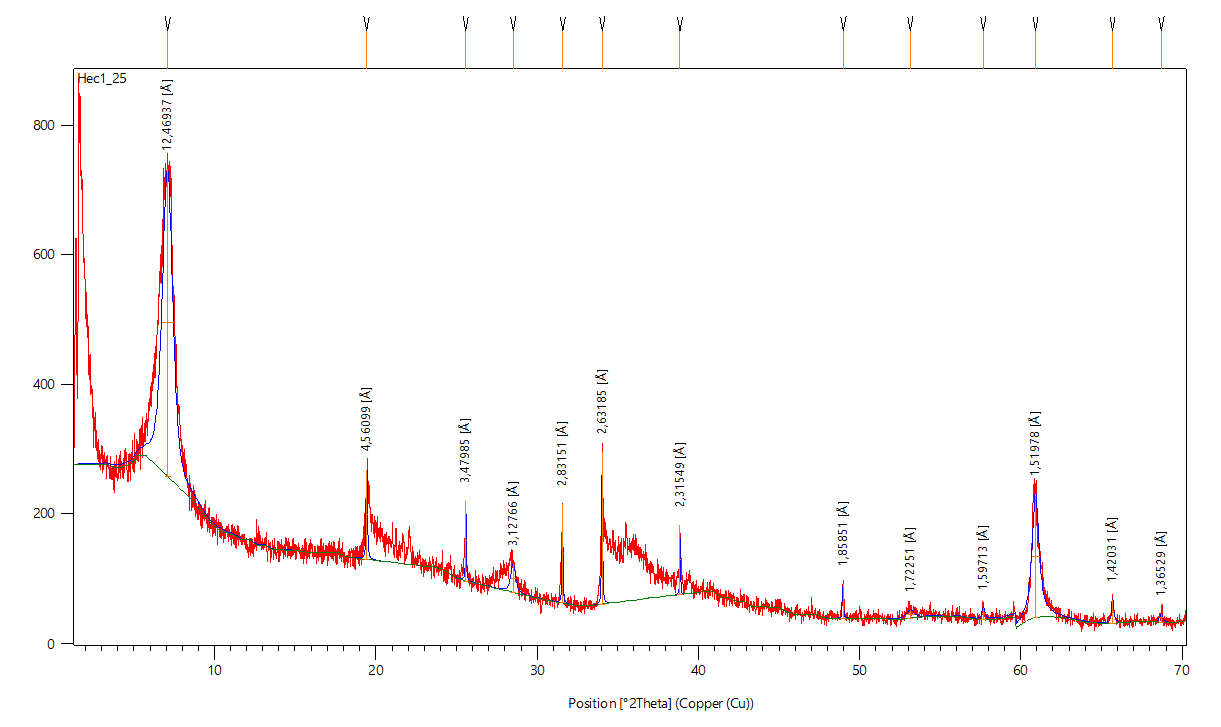
\includegraphics[scale=0.5]{Hec1.png}
  \caption{Zeigt das Pulverdiffraktogramm des Hectorits, dabei sind die Reflexe mit den Abstand der $d_{00n}$ Serie markiert.}
  \label{Hec1}
\end{figure}
\noindent
Aus Abbildung \ref{Hec1} ist ersichtlich, dass der $d_{001}$-Reflex bei einem Abstand von 12.46937 \AA liegt. 
Auf Grundlage dieses Werts lassen sich die theoretischen Abstände der $d_{00n}$-Serie berechnen. Dies erfolgt mithilfe der Formel \ref{d00n}.

\begin{equation}
  d_{00n}=\frac{d_{001}}{n}
  \label{d00n}
\end{equation}
\noindent
Die daraus erhaltenen Werte werden mit den in Abbildung \ref{Hec1} dargestellten experimentellen Daten verglichen und in Tabelle \ref{VergleichHec1} zusammengefasst.
\newpage
\begin{table}[h!]
\caption{\textit{Vergleich der aus Gleichung \ref{d00n} berechneten theoretischen Werte mit den experimentell bestimmten Werten aus Abbildung \ref{Hec1}.}}
\begin{center}
\begin{tabular}{|>{\columncolor{lightgray}}p{4cm}|>{\centering\arraybackslash}p{4cm}|>{\centering\arraybackslash}p{4cm}|}
   \hline
   \rowcolor{gray}
   &Berrechnete Werte& experimentellen Werte \\
   \hline
   $d_{001}$ [\AA]&12.46937& 12.46937\\
   \hline
   $d_{002}$ [\AA]&6.234685& Konnte nicht zugeordnet werden\\
   \hline
   $d_{003}$ [\AA]&4.156457& 4.56099\\
   \hline
   $d_{004}$ [\AA]&3.117343& 3.12766\\
   \hline
   $d_{005}$ [\AA]&2.493874& 2.63185\\
   \hline
   $d_{006}$ [\AA]&2.078228& 1.85851\\
   \hline

\end{tabular}
\label{VergleichHec1}
\end{center}
\end{table}
\noindent
Aus den experimentellen Werten in Tabelle \ref{d00n} wird der Mittelwert gemäß Formel \ref{Mittelwert} berechnet.
\begin{equation}
  \overline{d}=\frac{\sum_{i}^{n}d_{00i}\cdot i}{n}=12.595
  \label{Mittelwert}
\end{equation}
\noindent
Zur Berechnung des Variationskoeffizienten werden die Gleichungen \ref{CV1} und \ref{CV2} herangezogen.
Bei Gleichung \ref{CV1} werden die Werte von $d_{001}$ nicht berücksichtigt, da es sich bei dem „berechneten“ Wert, eigentlich um einen experimentellen Wert handelt.
\begin{equation}
  \sqrt{\frac{\sum_{i}^{n}(d_{00i \enspace experimentell} - d_{{00i}\enspace{berechnet}})^2}{n-1}} =
  \label{CV1}
\end{equation}
\begin{equation}
  \sqrt{2}
  \label{CV2}
\end{equation}





\newpage









\newpage
\section{Zusammenfassung}
\cite{Skript}



\newpage
\section{Literaturverzeichnis}
\printbibliography



\end{document}